\chapter{Abstract State Machines}

Le ASM sono delle FSM (\textit{Final State Machines}) con stati generalizzati; rappresentano la forma 
matematica di macchine che estendono la nozione di FSM, \textbf{ampliando la definzione di stato} 
e \textbf{modificando la forma delle transizioni}.

\subsubsection{Stati}
Gli stati di controllo non strutturati vengono sostituiti da stati (strutturati) che 
modellano:
\begin{itemize}
    \item \textbf{dati} complessi arbitrati (con domini di base e funzioni per la struttura)
    \item \textbf{operazioni} per la manipolazione di dati
\end{itemize}

\noindent Possiamo definire gli stati come delle \textit{algebre}.

\begin{figure}[H]
    \centering
    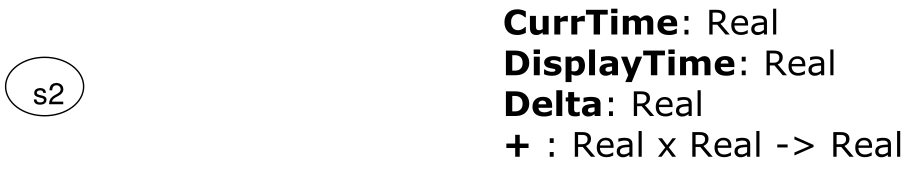
\includegraphics[width=0.8\linewidth]{chapters/1-asm/images/stati.png}
\end{figure}

\subsubsection{Transizioni}
Le transizione sono \textit{"regole"} che descrivono il cambiamento 
di funzioni da uno stato al successivo; permettono di modificare la 
struttura algebrica durante l'esecuzione della ASM.

\begin{center}
    \textit{if condition then Updates}
\end{center}

\noindent Negli FSM le transizioni sono rappresentate con delle frecce.

\newpage
Le ASM sono dotate di un ambiente di tool per:
\begin{itemize}
    \item editing
    \item simulazione
    \item validazione 
    \item verifica
    \item generazioni di casi di test
\end{itemize}

\noindent Un modello ASM può essere visto come pseudocodice su strutture dati astratte.

\subsubsection{Da FSM a ASM}
\begin{figure}[H]
    \centering
    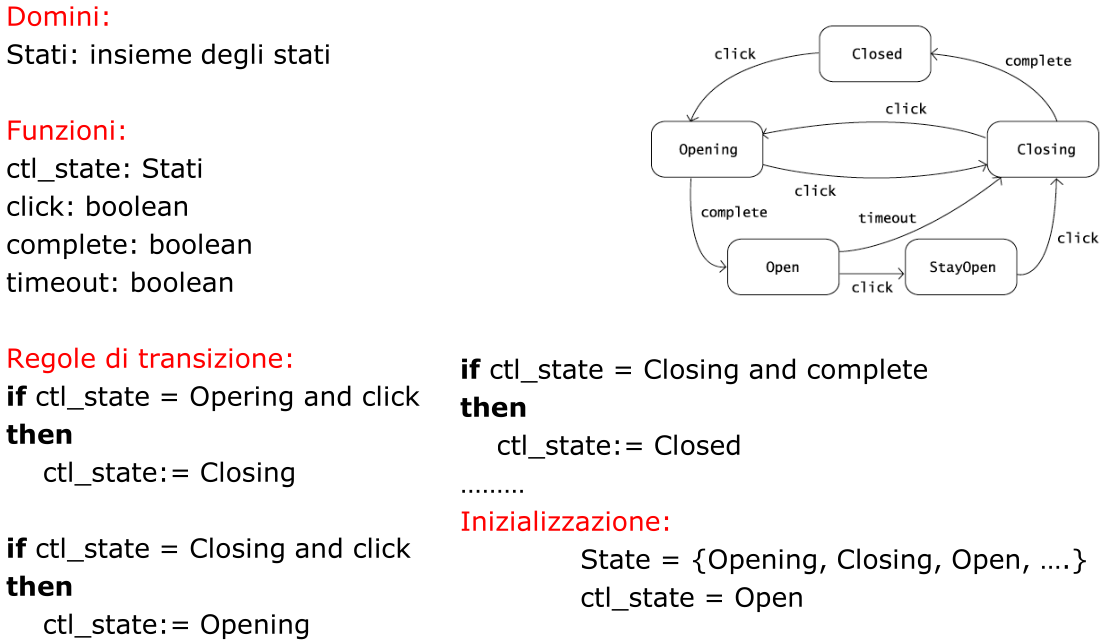
\includegraphics[width=0.92\linewidth]{chapters/1-asm/images/fsm-asm2.png}
\end{figure}

\noindent Possiamo definire ASM = (header, body, main rule, inizialization)

\begin{figure}[H]
    \centering
    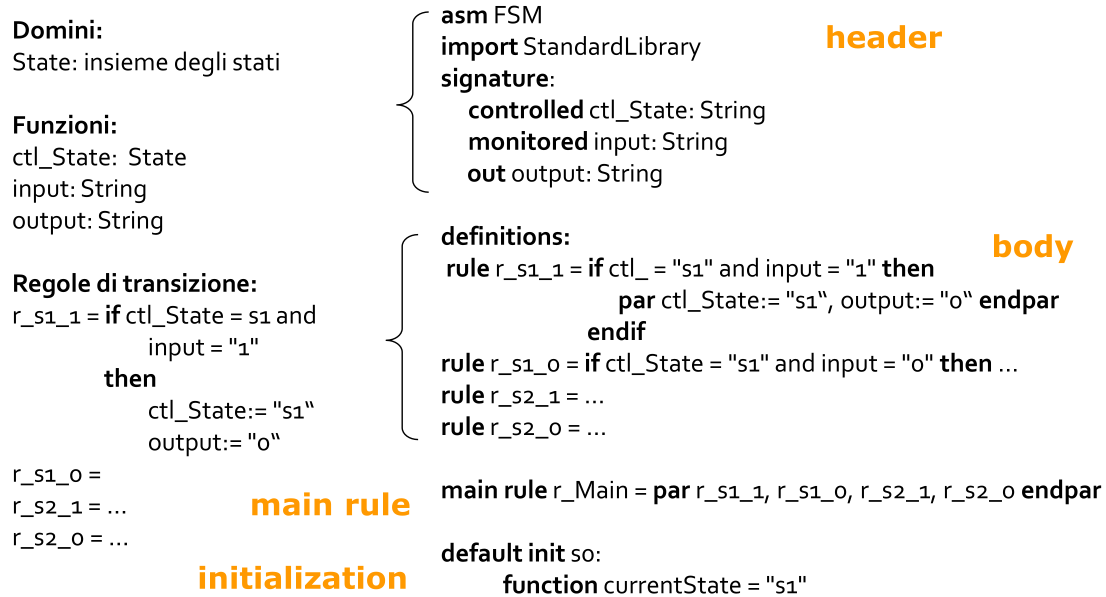
\includegraphics[width=0.92\linewidth]{chapters/1-asm/images/comp-asm.png}
\end{figure}

\section{Formalismo}

\subsection{Vocabolario}
\underline{\textbf{DEF:}} Un \textbf{vocabolario} $\Sigma$ è una collezione finita di nomi di 
funzioni.

\noindent Le funzioni possono essere dinamiche o statiche, a seconda che l'interpretazione 
del nome della funzione cambia o no da uno stato al successivo (funzioni 
in senso matematico).

\subsection{Costanti}
Le funzioni statiche di arietà zero sono dette \textbf{costanti}. Ogni 
vocabolario contiene sempre le costanti \textit{undef, true, false}.

\noindent Ad esempio:
\begin{itemize}
    \item i numeri sono costanti numeriche
    \item \texttt{voto = 30}
\end{itemize}


\subsection{Funzioni statiche}
Le funzioni statiche (arietà $>0$) sono definite tramite una legge fissa.

\noindent Ad esempio:
\begin{itemize}
    \item operazioni tra numeri (+, -, \dots)
    \item operazioni tra booleani (AND, OR, \dots)
    \item \texttt{max(m, n)}
\end{itemize}

\subsection{Fuzioni dinamiche}
Le funzioni dinamiche di arietà zero sono le variabili dei linguaggi 
di programmazione.

\subsection{Stato ASM}
\underline{\textbf{DEF:}} Fissato un vocabolario $\Sigma$, uno \textbf{stato} A del 
vocabolario $\Sigma$ è un insieme non vuoto $X$, detto \textit{superuniverso di A}, con 
le interpretazioni dei nomi delle funzioni di $\Sigma$.

\noindent Da questa definizione, segue che:
\begin{itemize}
    \item se $f$ è un nome di funzione \textit{n-aria} di $\Sigma$, allora 
    la sua interpretazione $f^A$ è una funzione da $X^n$ a $X$
    \item Se $c$ è un nome di costante di $\Sigma$, allora la sua interpretazione $c^A$ è un elemento di $X$
\end{itemize}

\noindent Possiamo definire il superuniverso come un \textit{"dominio di 
interpretazione"}; i simboli del vocabolario, presi singoralmente, sono soltanto simboli.

\subsection{Domini ASM}
Il superuniverso di uno stato ASM è suddiviso in \textit{universi}, 
rappresentati dalle loro funzioni caratteristiche.

\begin{center}
    \textit{Se A è un sottoinsieme dell'insieme X, la funzione caratteristica di A è quella 
    funzione da X all'insieme $\{0 , 1\}$ che sull'elemento x $\in$ X vale 1 se x appartiene ad A, e vale 0 in caso contrario.  }
\end{center}

\noindent Ogni universo rappresenta un dominio. In base a questa 
rappresentazione degli insiemi in termini di funzioni caratteristiche, uno stato di una 
ASM consente di modellare \textbf{domini eterogenei}.

\noindent Alcuni esempi di domini:
\begin{itemize}
    \item predefiniti, come \texttt{Interi, String, \dots}
    \item definiti dall'utente, come tipi astratti o a partire da altri domini
\end{itemize}

\subsubsection{Esempio}
Dominio $X=\{1,2,a,b,mario,pippo\}$, ripartito in domini:
\begin{itemize}
    \item $Interi = \{1.2\}$
    \item $Char = \{a,b\}$
    \item $String = \{mario, pippo\}$
\end{itemize}

\subsection{Termini ASM}
\underline{\textbf{DEF:}} i termini di $\Sigma$ sono espressioni sintattiche così costruite:
\begin{enumerate}
    \item Variabili $v_0, v_1, v_2, \dots$ sono termini 
    \item Costanti $c$ di $\Sigma$ sono termini 
    \item Se $f$ è un nome di funzione \textit{n-aria} di $\Sigma$ e 
    $t_1, \dots, t_n$ sono termini 
    
    $\Rightarrow f(t1, \dots, t_n)$ è un termine 
\end{enumerate}

\noindent Ad esempio:
\begin{itemize}
    \item $v_0 + v_1$
    \item $1 + (v_2 * 0)$
\end{itemize}

\noindent Un termine che non contiene variabili è detto chiuso. I termini 
sono \textit{oggetti sintattici}. \textbf{Assumono significato (o semantica)
nello stato}; il suo valore è l'\textit{interpretazione del termine} in $A$.

\newpage
\section{Regole di transizione ASM}
\textbf{Aggiornare stati astratti} significa cambiare interpretazione delle 
(o solo di alcune) funzioni della segnatura della macchina. Il modo in cui la macchina 
aggiorna il proprio stato è descritto da \textbf{regole di transizione}; l'insieme 
delle regole di transizione definiscono la sintassi di un \textit{programma ASM}.

\noindent Le regole sono \textit{espressioni sintattiche generate su $\Sigma$} attraverso 
l'uso di \textbf{costruttori di regole} 

\subsection{Update rule}

$f(t_1, \dots, t_n) := s$, dove:
\begin{itemize}
    \item $f$ è un nome di funzione \textbf{dinamica} \textit{n-aria} di $\Sigma$
    \item $(t_1, \dots, t_n)$ e $s$ sono termini di $\Sigma$
\end{itemize}

\noindent Significa che nello stato successivo, il valore di $f$ per gli 
argomenti $(t_1, \dots, t_n)$ è aggiornato ad $s$. Nel caso di una funzione 0-aria, 
cioè una variabile $x$, l'aggiornamento ha la forma $x := s$


\subsubsection{Locazione ASM}
Una locazione è definita matematicamente come una coppia $(f, (v_1, \dots, v_n))$ con 
$f$ nome di funzione e $(v_1, \dots, v_2)$ i suoi argomenti.

\noindent In uno stato $S$, una locazione ha un \textit{valore}: l'interpretazione del 
della funzione nello stato. Una funzione può essere: 
\begin{itemize}
    \item Variabile (0-arie): x, y, \dots
    \item Funzioni (n-arie): f(1), name(2), \dots
\end{itemize}


\subsubsection{Aggiornamento di locazione}

Le transizioni di stato delle ASM, tramite update rule, causano \textbf{aggiornamenti}
dei valori contenuti nelle locazioni.

\noindent Se $loc = (f,(v_1, \dots, v_n))$ e $loc = a$, l'aggiornamento di $loc$ ha la forma:

$f(v_1, \dots, v_2) := newval$

\subsection{Costruttore if-then-else}

\texttt{if $\phi$ then R else S}, ovvero: \textit{se $\phi$ è vera, allora esegui $R$, altrimenti
esegui $S$}.

\begin{figure}[H]
    \centering
    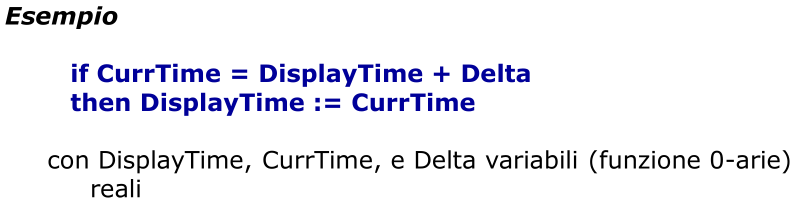
\includegraphics[width=0.8\linewidth]{chapters/1-asm/images/ex1.png}
\end{figure}

\subsection{Classificazione delle funzioni}

\noindent Sia $M$ una ASM e $env$ l'ambiente di $M$:
\begin{itemize}
    \item \textbf{Dynamic}
    \begin{itemize}
        \item \textit{monitored:} lette (non aggiornate) da $M$, scritte da $env$
        
        \texttt{CurrTime} viene incrementato dall'esterno
        \item \textit{out:} scritte (non lette) da $M$, lette da $env$
        \item \textit{controlled:} lette e scritte da $M$
        
        \texttt{DisplayTime} viene incrementato dalla regola
        \item \textit{shared:} lette e scritte da $M$ e $env$  
    \end{itemize}
    \item \textbf{Derived:} valori computati da funzioni monitorate e funzioni statiche 
    per mezzo di una "legge" fissata a priori 
\end{itemize}

\begin{figure}[H]
    \centering
    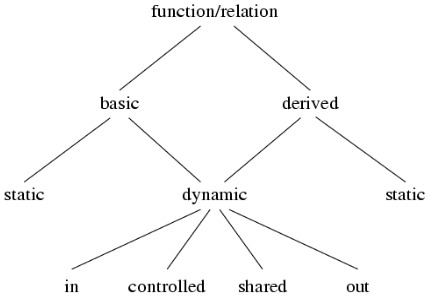
\includegraphics[width=0.7\linewidth]{chapters/1-asm/images/classificazione-funzioni.png}
\end{figure}

\subsection{Costruttore skip}
\begin{figure}[H]
    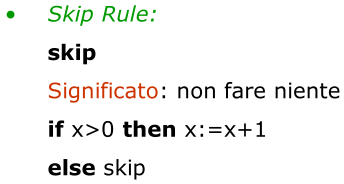
\includegraphics[width=0.4\linewidth]{chapters/1-asm/images/skip.png}
\end{figure}

\newpage
\subsection{Costruttore let}
Serve per abbreviare ad esempio un termine molto complesso o lungo. 

\begin{figure}[H]
    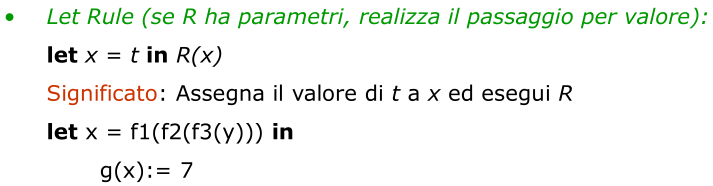
\includegraphics[width=0.8\linewidth]{chapters/1-asm/images/let.png}
\end{figure}

\subsection{Costruttore "par" per block rule}

\begin{figure}[H]
    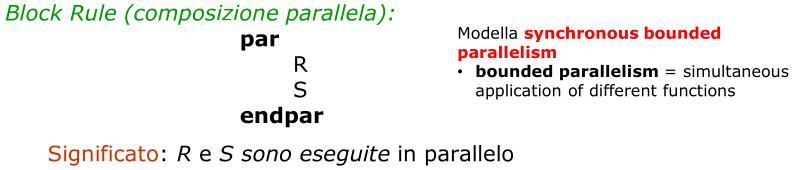
\includegraphics[width=0.8\linewidth]{chapters/1-asm/images/par.png}
\end{figure}

\section{Aggiornamenti consistenti}
A causa del parallelismo, una regola di transizione può richiedere 
\textbf{più volte l'aggiornamento di una stessa funzione} per gli 
stessi argomenti. Si richiede che tali aggiornamenti siano \textbf{consistenti}.

\noindent Data la funzione $f(a_1, \dots, a_n)$ in uno stato $S_i$ della macchina:
\begin{itemize}
    \item La coppia $loc = (f, (a_1, \dots, a_n))$ è detta \textit{locazione} e rappresenta
    matematicamente il valore di $f(a_1, \dots, a_n)$ in memoria 
    \item Un \textit{aggiornamento} è la coppia $(loc, b)=((f,(a_1,\dots,a_n)), b)$
    
    $\rightarrow$ significa che l'interpretazione della funzione $f$ in $S_i$ viene modificata 
    per gli argomenti $a_1, \dots, a_n$ con il valore $b$ in $S_{i+1}$
    \item Un \textbf{update set} è un insieme di aggiornamnti
\end{itemize}


\noindent \underline{\textbf{DEF:}} Un update set $U$ è \textbf{consistente}
se vale:

\noindent $\forall$ locazione $(f, (a_1, \dots, a_n))$, se:
\begin{itemize}
    \item $(f, (a_1, \dots, a_n)) \in U$
    \item $(f, (a_1, \dots, a_n)) \in U$ 
    \item $\Rightarrow b = c$
\end{itemize}


\noindent Se $b \neq c$, allora l'update si dice \textbf{inconsistente} (stiamo scrivendo 
due valori diversi nella stessa locazione).

\begin{itemize}
    \item Se l'update set è consistente, allora i suoi aggiornamenti possono 
    essere eseguiti in un dato stato; il risultato è un nuovo stato dove le 
    \textit{interpretazioni} dei nomi di \textit{funzioni dinamiche} sono cambiati 
    secondo $U$
    \item Le \textit{interpretazioni} dei nomi delle\textit{funzoni statiche} sono gli stessi 
    dello stato precedente 
    \item le \textit{interpretazioni} dei nomi delle \textit{funzioni monitorate} sono date dall'ambiente esterno 
    e possono dunque cambiare in modo arbitrario
\end{itemize}


\section{Rule construnctor}

\begin{figure}[H]
    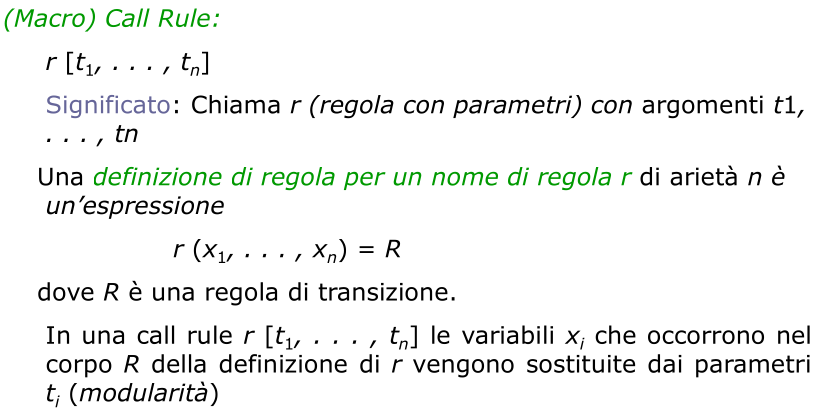
\includegraphics[width=0.8\linewidth]{chapters/1-asm/images/call-rule.png}
\end{figure}







